%%===============================================================================
% Document configuration

%%-------------------------------------------------------------------------------
% Document type
\documentclass[utf8]{FrontiersinHarvard}

%%-------------------------------------------------------------------------------
% Package configuration
\usepackage                                                                     % LaTeX Packages
{
    amsmath,                                                                    % Miscellaneous enhancements for mathematics
    amssymb,                                                                    % Math symbols
    booktabs,                                                                   % Extend tables
    cite,                                                                       % Improved citation mechanics
    graphicx,                                                                   % Enhance graphics
    lineno,                                                                     % Add line numbers to page
    microtype,                                                                  % Uses different techniques for spacing
    multicol,                                                                   % Create tables spanning multiple columns
    multirow,                                                                   % Create tables spanning multiple rows
    pgfplots,                                                                   % Plot in LaTeX
    subcaption,                                                                 % Subfigures (Get rid of this)
    subfloat,                                                                   % Subfigures
    tabularx,                                                                   % Add more contol to tables
    tikz,                                                                       % Generate figures in LaTeX
    xcolor,                                                                     % Colors
    xfp,                                                                        % No trailing zeros
}

%% Plot configurations
\usetikzlibrary{automata, positioning, arrows.meta}                             % Tikz macros
\pgfplotsset{compat=1.3, width=\textwidth}
\graphicspath{ {./fig/} }                                                       % Paths to find images

%% Paper configuration
\linenumbers                                                                    % Put line numbers
\setlength{\columnsep}{2cm}                                                     % Column separation
\let\cite\citep                                                                 % Redefine `\cite` as `\citep` because lazy

%%-------------------------------------------------------------------------------
% Custom Commands
\newcommand{\TODO}[1]{{\color{green} To do: #1}}                                % For adding notes to paper
\def\keyFont{\fontsize{8}{11}\helveticabold }

% Experiment information
%% Experiment parameters
\newcommand{\A}{35 }                                                            % Number of buses
\newcommand{\N}{338 }                                                           % Number of visits
\newcommand{\acharge}{0.9}                                                      % BOD charge percentage
\newcommand{\bcharge}{0.7 }                                                     % EOD charge percentage
\newcommand{\mincharge}{25\% }                                                  % Min visit charge percent
\newcommand{\maxcharge}{100\% }                                                 % Max visit charge percent
\newcommand{\batsize}{388 }                                                     % Battery capacity
\newcommand{\fast}{15 }                                                         % Number of fast chargers
\newcommand{\slow}{15 }                                                         % Number of slow chargers
\newcommand{\fasts}{911 }                                                       % Speed of fast charger
\newcommand{\slows}{30 }                                                        % Speed of slow charger

%% Solve output
\newcommand{\timeran}{14400 }                                                   % Time ran for MILP
\newcommand{\gappercent}{52.5\% }                                               % Gap percent after runtime
\newcommand{\processor}{Ryzen 9 }                                               % Processor type

%%-------------------------------------------------------------------------------
% Authors
\def\keyFont{\fontsize{8}{11}\helveticabold }
\def\firstAuthorLast{Brown {et~al.}} %use et al only if is more than 1 author
\def\Authors{Alexander Brown\,$^{1,*}$, Greg Droge\,$^{1}$, Jacob Gunther\,$^{1}$}
% Affiliations should be keyed to the author's name with superscript numbers and be listed as follows: Laboratory,
% Institute, Department, Organization, City, State abbreviation (USA, Canada, Australia), and Country (without detailed
% address information such as city zip codes or street names). If one of the authors has a change of address, list the
% new address below the correspondence details using a superscript symbol and use the same symbol to indicate the author
% in the author list.
\def\Address{$^{1}$Department of Electrical and Computer Engineering, Logan, UT, USA}
% The Corresponding Author should be marked with an asterisk Provide the exact contact address (this time including
% street name and city zip code) and email of the corresponding author
\def\corrAuthor{Alexander Brown}
\def\corrEmail{A01704744@usu.edu}

\author[\firstAuthorLast ]{\Authors} %This field will be automatically populated
\address{} %This field will be automatically populated
\correspondance{} %This field will be automatically populated
\extraAuth{}

%%===============================================================================
% Title, Authors, Abstract, Keywords
\begin{document}
\onecolumn
\firstpage{1}

%%-------------------------------------------------------------------------------
% Title
\title{A Position Allocation Approach to the Scheduling of Battery Electric Bus Charging}

%%---------------------------------------------------------------------------------
% Create title
\maketitle

%%---------------------------------------------------------------------------------
% Abstract
\begin{abstract}
Robust charging schedules for an increasing interest of battery electric bus (BEB) fleets is a critical component to
a successful adoption. In this paper, a BEB charging scheduling framework that considers spatiotemporal schedule
constraints, route schedules, fast and slow charging, and battery charging dynamics is modeled as a mixed integer linear
program (MILP). The MILP is modeled after the berth allocation problem (BAP) in a modified form known as the position
allocation problem (PAP). Linear battery dynamics are included to model the charging and discharging of buses while at
the station and during their routes, respectively. The optimization coordinates BEB charging to ensure each BEB has
sufficient charge while using slow chargers where possible for sake of battery health. The model also minimizes the
total number of chargers utilized and prioritizes slow chargers. The model validity is demonstrated with a set of routes
sampled from Utah Transit Authority (UTA) for \A buses and \N visits to the charging station. The model is also compared
to a heuristic based algorithm, referred to as the Quin-Modified method. The results presented show that the slow
chargers are more readily selected and the charging and spatiotemporal constraints are met while considering the battery
dynamics, minimizing the charger count, and consumption cost.

\tiny \keyFont{ \section{Keywords:} Berth Allocation Problem (BAP), Position Allocation Problem (PAP), Mixed Integer
  Linear Program (MILP), Battery Electric Bus (BEB), Scheduling} %All article types: you may provide up to 8 keywords;
at least 5 are mandatory.
\end{abstract}

%%===============================================================================
% Paper

%%-------------------------------------------------------------------------------
% Introduction
\section{Introduction}
\label{sec:introduction}
The public transportation system is crucial in any urban area; however, the increased awareness and concern of
environmental impacts of petroleum based public transportation has driven an effort to reduce the pollutant footprint
\cite{DeFilippo2014, Xylia2018, Guida2017, Li2016}. Particularly, the electrification of public bus transportation via
battery power, i.e., battery electric buses (BEBs), has received significant attention \cite{Li2016}. Although the
technology provides benefits beyond reduction in emissions, such as lower driving costs, lower maintenance costs, and
reduced vehicle noise, battery powered systems introduce new challenges such as larger upfront costs, and potentially
several hours long ``refueling'' periods \cite{Xylia2018, Li2016}. Furthermore, the problem is exacerbated by the
constraints of the transit schedule to which the fleet must adhere, the limited amount of chargers available, and the
adverse affects in the health of the battery due to fast charging \cite{Lutsey2019}. This paper presents a continuous
scheduling framework for a BEB fleet that shares limited fast and slow chargers. This framework takes into consideration
linear charging dynamics and a fixed bus schedule while meeting a certain battery charge threshold throughout the day.

Many recent efforts have been made to simultaneously solve the problems of route scheduling, and charging fleets and determining
the infrastructure upon which they rely, e.g., \cite{Wei2018, Sebastiani2016, Hoke2014, Wang2017}. Several simplifications
are made to make these problems computationally feasible \todo{citations}. These simplifications to the charge
scheduling model include utilizing only fast chargers while planning \cite{Wei2018, Sebastiani2016, Wang2017,
  Zhou2020-0, Liu2020, Yang2018, Wang2017a, Qin2016}. If slow chargers are used, they are only employed at the depot and
not the station \cite{He2020, Tang2019}. Some approaches also simplify by assuming a full charge is always achieved \cite{Wei2018, Wang2017, Zhou2020-0,
  Wang2017a}. Others have assumed that the charge received is proportional to the time spent on the charger
\cite{Liu2020, Yang2018}, which can be a valid assumption when the battery state-of-charge (SOC) is below 80\% charge
\cite{Liu2020}.

This work builds upon the Position Allocation Problem \cite{Qarebagh2019}, a modification of the well studied Berth Allocation Problem
(BAP), as a means to schedule the charging of electric vehicles \cite{Buhrkal2010, Frojan2015, Imai2001}.
The BAP is a continuous time model that solves the problem of allocating space for incoming vessels to be berthed. Each
arriving vessel requires both time and space to be serviced and is assigned a berthing location \cite{Imai2001}. Vessels
are lined up parallel to the berth to be serviced and are horizontally queued as shown in Fig \ref{subfig:bapexample}.
The PAP utilizes this notion of queuing for scheduling vehicles to be charged, as shown in Fig \ref{subfig:papexample}.
The PAP is formulated as a rectangle packing problem by assuming that vehicle charging will take a fixed amount of time,
the amount of vehicles that can charge is limited by the physical width of the vehicles, and each vehicle visits the
charger a single time \cite{Qarebagh2019}.

The main contribution of this work is the extension of the PAP novel approach to BEB charger scheduling. This includes
modeling and incorporation of a proportional charging model into the MILP framework, consideration of multiple charger
types, and inclusion of the route schedule for each bus. The last contribution is of importance because both the BAP and PAP
consider each arrival to be unique; thus, a method of tracking buses must be implemented.
The result is a MILP formulation that coordinates charging times and charger type for every visit that each bus makes to the station while considering a dynamic charge model and
scheduling constraints.

The remainder of the paper proceeds as follows: In Section \ref{sec:positionallocationproblem}, the PAP is introduced
with a formulation of the resulting MILP. Section \ref{sec:problemformulation} constructs the MILP for BEB scheduling,
including modifications to the PAP queuing constraints and development of a dynamic charging model. Section
\ref{sec:example} demonstrates an example of using the formulation to coordinate \A buses over \N total visits to the
  station. The paper ends in Section \ref{sec:conclusion} with concluding remarks.

%%-------------------------------------------------------------------------------
% The Position Allocation Problem
\section{The Position Allocation Problem}
\label{sec:positionallocationproblem}
This section provides a brief overview of the BAP and a detailed formulation of PAP as presented in \cite{Qarebagh2019}.

\subsection{Overview of BAP}
The BAP is a rectangle packing problem where a set
of rectangles ($\mathbb{O}$) are attempted to be optimally placed in a larger rectangle ($O$) as shown in Fig
\ref{fig:packexample}. The rectangle packing problem is an NP-hard problem that can be used to describe many real life
problems \cite{Bruin2013,Murata1995}. In some of these problems, the dimensions of $\mathbb{O}$ are held constant such
as in the problem of packing modules on a chip, where the widths and height of the rectangles represent the physical
width and heights of the modules \cite{Murata1995}. Other problems, such as the BAP can allow one side of
the rectangle to vary depending on its assigned position (e.g. the handling time is dependent on the berth)
\cite{Buhrkal2010}.

The BAP solves the problem of optimally assigning incoming vessels to berth positions to be serviced (Fig
\ref{subfig:bapexample}). The width and height of $O$ represent the berth length $S$ and time horizon $T$, respectively.
Similarly, the width and height for $\mathbb{O}$ represent the time spent to service vessel $i$ and the space taken by
docking vessel $i$, respectively. The vessel characteristics (length of the vessel, arrival time, handling time, desired
departure time) are assumed to be known for all $N$ vessels to be serviced. A representation of a BAP solution is shown
in Fig \ref{fig:bap}.

\subsection{The PAP Formulation}
The BAP forms the basis of the PAP; however, there are some differences in the way the variables are
perceived. For the $i^{th}$ visit, starting service time, $u_i$, is now the starting charge time, the berth location,
$v_i$, is now the charger queue for assignment, and the service time, $p_i$, is now the time to charge. There are also a few
key concepts on the model. The PAP models the set of chargers as one continuous line. In order to define distint chargers, the 
line is discrtized into $n_Q$ queues with a unit length of 1 and \todo{charge rate} of $r_q$. The charge times are continuous and 
can be placed anywhere on the time horizon, $[0,T]$, as long as the allocated times do not interfere with other scheduled charge times.
The PAP utilizes a number of parameters. The following parameters are constants. 

\begin{itemize}
	\item $n_Q$ : total number of chargers
	\item $T$   : 
	\item $n_V$ : total number of incoming vehicles
	\item $p_i$ : charging time for vehicle $i;\; 1 \leq i \leq N$
	\item $s_i$ : width of vehicle $i;\; 1 \leq i \leq N$
	\item $a_i$ : arrival time of vehicle $i;\; 1 \leq i \leq N$
\end{itemize}

These constants define the problem bounds. The following list provides a series of decision variables used in the
formulation.

\begin{itemize}
    \item $u_i$    : starting charge time for vehicle $i;\; 1 \leq i \leq N$
    \item $v_i$    : assigned charge queue for vehicle $i;\; 1 \leq i \leq N$
    \item $c_i$    : departure time for vehicle $i;\; 1 \leq i \leq N$
    \item $\sigma_{ij}$ : binary variable that determines ordering of vehicles $i$ and $j$ in time
    \item $\delta_{ij}$ : binary variable that determines relative position of vehicles $i$ and $j$ when charging simultaneously
\end{itemize}

To determine the values for each of these decision variables, a MILP is formulated in \cite{Qarebagh2019} and shown
here for sake of completeness.

\begin{equation}
	\label{eq:bapobjective}
	\min\; \sum_{i=1}^N (c_i - a_i)
\end{equation}
Subject to:
\begin{subequations}
\label{eq:bapconstrs}
\begin{align}
    u_j - u_i - p_i - (\sigma_{ij} - 1)T \geq 0                  \label{subeq:baptime}          \\
    v_j - v_i - s_i - (\delta_{ij} - 1)Q \geq 0                  \label{subeq:bapspace}         \\
    \sigma_{ij} + \sigma_{ji} + \delta_{ij} + \delta_{ji} \geq 1 \label{subeq:bapvalid_pos}     \\
    \sigma_{ij} + \sigma_{ji} \leq 1                              \label{subeq:bapsigma}        \\
    \delta_{ij} + \delta_{ji} \leq 1                              \label{subeq:bapdelta}        \\
    p_i + u_i = c_i                                               \label{subeq:bapdetach}       \\
    a_i \leq u_i \leq (T - p_i)                                   \label{subeq:bapvalid_starts} \\
    \sigma_{ij} \in \{0,1\},\;\delta_{ij} \in \{0,1\}\;           \label{subeq:bapsdspace}      \\
    v_i \in [0 \mbox{ } S ]                                       \label{subeq:bapvspace}
\end{align}
\end{subequations}

\noindent

The objective function \eqref{eq:bapobjective} minimizes the time spent to service each vehicle by minimizing over the
sum of differences between the departure time, $c_i$, and arrival time, $a_i$. i.e., It seeks to get each vehicle
charged and on its way as quickly as possible.

Constraints \ref{subeq:baptime}-\ref{subeq:bapdelta} are used to ensure that individual rectangles do not overlap. For
the PAP, they ensure that two vehicles charging simultaneously are at different positions and, similarly, two vehicles
that have overlapping positions do not overlap temporally. Constraint \eqref{subeq:baptime} establishes temporal
ordering when active ($\sigma_{ij}=1$). Similarly, when $\delta_{ij} =1$ in \eqref{subeq:bapspace} then spatial ordering is
established. Constraints \ref{subeq:bapvalid_pos}-\ref{subeq:bapdelta} enforce that spatial and/or temporal ordering is
established between each possible vehicle pair. Constraints \eqref{subeq:bapsigma} and \eqref{subeq:bapdelta} enforce
consistency. For example, \eqref{subeq:bapsigma} enforces that vehicle $i$ cannot come before vehicle $j$ and vehicle
$j$ simultaneously come before vehicle $i$.

The last constraints force relationships between arrival time, charge start time, and departure time. Constraint
\eqref{subeq:bapdetach} states that the service start time, $u_i$, plus the time to service vehicle $i$, $p_i$, must
equal the departure time, $c_i$. Constraint \eqref{subeq:bapvalid_starts} enforces the arrival time, $a_i$, to be less
than or equal to the service start time, $u_i$, which in turn must be less than or equal to the latest time the vehicle
may begin to be serviced to stay within the time horizon. Constraint \eqref{subeq:bapsdspace} ensures that $\sigma_{ij}$ and
$\delta_{ij}$ are binary. Constraint \eqref{subeq:bapvspace} ensures that the assigned value of $v_i$ is a valid charging
position.

%%-------------------------------------------------------------------------------
%
\section{A Rectangle Packing Formulation for BEB Charging}  \label{sec:problemformulation}
Applying the PAP to BEB charging requires four fundamental changes. The first is that the time that a BEB spends
charging is allowed to vary. Thus, $p_i$ becomes a variable of optimization. Second, in the PAP each charging visit is
assumed to be a different vehicle. For the BEB charging problem, each bus may make multiple visits to the station
throughout the day and the resulting charge for a bus at a given time is dependent upon each of the prior visits made.
Third, in the PAP, the charger is one continuous bar with vehicle width effectively restricting the number of vehicles
charging simultaneously. For the BEB, it is assumed that a specific number of chargers exist, and these chargers can
charge the vehicle at a different rate. The fourth fundamental change is related to the first three. The charge of each
bus must be tracked in the optimization to ensure that charging across multiple visits is sufficient to allow each bus
to execute its route throughout the day.

The discussion of the four changes are separated into two sections. Section \ref{sec:queuing} discusses the changes in
the spatial-temporal constraint formulation to form a queuing constraint. Section \ref{sec:batt_dynamics} then discusses
the addition of the bus charge management. This section ends with a brief discussion of a modified objective in Section
\ref{sec:objective-function} and the statement of the full problem in Section \ref{sec:BEB_MILP}. The notation is
explained throughout and summarized in Table \ref{tab:variables}.

\subsection{Queuing Constraints} \label{sec:queuing}
\noindent
The queuing constraints help to ensure that the busses enter queues for charging or waiting as they come into the
station. There are three sets to differentiate between different entities. $\mathbb{B} = \{1, ..., n_B\}$ is the set of
bus indices with index $b$ used to denote an individual bus, $\mathbb{Q} = \{1, ..., n_Q\}$ is the set of queues with index $q$
used to denote an individual queue, and $\mathbb{V} = \{1, ..., n_V\}$ is a set of visits to the station with $i,j$ used
to refer to individual visits. The mapping $\Gamma: \mathbb{V} \rightarrow \mathbb{B}$ is used to map a visit index to a bus index with
the shorthand $\Gamma_i$ used to refer to the bus index for visit $i$.

Most variables are now defined in terms of a visit. Two separate visits could correspond to different buses or visits by
the same bus. The spatial variable $s_i$ is removed and $v_i$ is made to be an integer corresponding to which queue
visit $i$ will be using. Thus, when $\delta_{ij} = 1$, the visits must be at different chargers, i.e., $v_i-v_j \geq 1$. The
variable $S$ is likewise replaced with $n_Q$. Note that $n_Q = n_B + n_C$, where $n_B$ is the number of busses and $n_C$
is the number of chargers. The rationale for having extra queues is to allow buses to sit idle instead of charging. The
modified queuing constraints can be written as follows.

\begin{subequations}
\label{eq:packconstrs}
\begin{align}
    u_i - u_j - p_j - (\sigma_{ij} - 1)T \geq 0   \label{subeq:time}         \\
    v_i - v_j - (\delta_{ij} - 1)n_Q \geq 1       \label{subeq:space}        \\
    \sigma_{ij} + \sigma_{ji} + \delta_{ij} + \delta_{ji} \geq 1 \label{subeq:valid_pos}    \\
    \sigma_{ij} + \sigma_{ji} \leq 1                   \label{subeq:sigma}        \\
    \delta_{ij} + \delta_{ji} \leq 1                   \label{subeq:delta}        \\
    p_i + u_i = c_i                       \label{subeq:detach}       \\
    a_i \leq u_i \leq (T - p_i)                 \label{subeq:valid_starts} \\
    c_i \leq \tau_i                             \label{subeq:valid_depart} \\
    p_i \geq 0                               \label{subeq:pos_charge} \\
    \sigma_{ij} \in \{0,1\},\;\delta_{ij} \in \{0,1\}   \label{subeq:sdspace}      \\
    v_i \in \mathbb{Q}                               \label{subeq:vspace}
\end{align}
\end{subequations}

Constraints \eqref{subeq:time}-\eqref{subeq:valid_starts} and \eqref{subeq:sdspace} are nearly identical to those
described in Section \ref{sec:positionallocationproblem} with the sole change in \eqref{subeq:space} being described
above to conform to a queue. Constraint \eqref{subeq:valid_depart} is added to ensure that the ending charge time,
$c_i$, must be less than or equal to the required departure time from the station, $\tau_i$. This enables the bus schedules
to be considered during optimization. Finally, \eqref{subeq:vspace} enforces $v_i$ to be an integer in the set of
possible queues.

\subsection{Battery Charge Dynamic Constraints}
\label{sec:batt_dynamics}
Using purely the constraints in \eqref{eq:packconstrs} with the objective in \eqref{eq:bapobjective} would result in
$c_i$ being chosen as small as possible by employing $p_i = 0,\; u_i = c_i$. Thus, the vehicles would not charge.
Furthermore, it does not encode any revisiting of the BEB to the charging station. To remedy this, battery dynamic
constraints are introduced.

Battery charge dynamic constraints are used to model the charge in each bus with the purpose of ensuring sufficient time
is spent charging. Two constraints are enforced on the bus charge: busses must always have sufficient charge to execute
their respective routes and each bus must end the day with a specific charge threshold, preparatory to execution for the
next day.

The charge at the beginning of visit $i$ is denoted as $\eta_i$. As a charge on the bus is dependent upon the visits that
bus makes to the station, the mapping $\Upsilon: \mathbb{V} \rightarrow \mathbb{V} \bigcup \{\varnothing\}$ is used to determine the next visit
that corresponds to the same bus, with $\Upsilon_i$ being shorthand notation. Thus, $\Gamma_i$ and $\Gamma_{\Upsilon_i}$ would both map to the
same bus index as long as $\Upsilon_i$ is not the null element, $\varnothing$. The null element is used to denote that there
are no future visits by that same bus.

To drive time spent on the charger, $p_i$, as well as define initial, final, and intermediate bus charges for each visit
$i$, the sets for initial and final visits must be defined. Let the mapping of the first visit by each bus be denoted as
$\Gamma^0_i : \mathbb{V} \rightarrow \mathbb{V} \bigcup \{\varnothing \}$. The indexed value of $\Gamma^0_i$ represents the index for the first
visit of bus $b$ or the null element, $\varnothing$. Similarly, let $\Gamma^f_i : \mathbb{V} \rightarrow \mathbb{V} \bigcup \{\varnothing \}$
contain the indexes for the final visit of each bus $b$ or the null element. The initial and final bus charges can then
be represented by the constraint equations $\eta_{\Gamma^0_i} = \alpha \kappa_{\Gamma^0_i}$ and \(\eta_{\Gamma^f_i} = \beta \kappa_{\Gamma^f_i}\), respectively,
where $\alpha$ and $\beta$ are percentages of the battery for first and final visit, respectively. The intermediate charges must
be determined at solve time.

It is assumed that the charge received is proportional to the time spent charging. The charge rate for charger $q$ is
denoted as $r_q$. Note that a value of $r_q = 0$ corresponds to a queue where no charging occurs. A bus in such a queue
is simply waiting for the departure time. Thus, $n_Q = n_C + n_B$ where the final $n_B$ queues have $r_q = 0$ to allow
an arbitrary number of buses to not charge at any given moment in time. The amount of discharge between visits $i$ and
$\Upsilon_i$, the next visit of the same bus, is denoted as $\lambda_i$. If visit $i$ occurred at charger $q$, the charge of the bus
coming into visit $\Upsilon_i$ would be

\begin{equation}
	\eta_{\Upsilon_i} = \eta_i + p_i r_q - \lambda_i.
\end{equation}

The binary decision variable $w_{iq}$ is introduced to determine whether visit $i$ uses charger $q$. This allows the
charge of the bus coming into visit $\Upsilon_i$ to be written in summation form as

\begin{subequations}
    \label{subeq:pre_next_charge}
\begin{align}
    \eta_{\Upsilon_i} = \eta_i + \sum_{q=1}^{n_Q} p_i w_{iq} r_q - \lambda_i  \\
    \sum_{q=1}^{n_Q} w_{iq} = 1 \\
    w_{iq} \in \{0,1\}
\end{align}
\end{subequations}

The choice of queue for visit $i$, $v_i$, becomes a slack variable and is defined in terms of $w_{iq}$ as

\begin{equation}
    v_i = \sum_{q=1}^{n_Q} qw_{iq}
\end{equation}

Maximum and minimum values for the charges are included to ensure the battery is not overcharged and to guarantee
sufficient charge for subsequent visits. The upper and lower battery charge bounds for bus $b$ are $\kappa_b$ and $\nu_b$,
respectively. As $\eta_i$ corresponds to the charge at the beginning of the visit, the upper bound constraint must also
include the charge received during the visit as follows.

\begin{subequations}
    \label{subeq:pre_min_max}
\begin{align}
    \eta_i + \sum_{q=1}^{n_Q} p_i w_{iq} r_q \leq \kappa_{\Gamma_i}                 \\
    \eta_i \geq \nu_{\Gamma_i} \kappa_{\Gamma_i}
\end{align}
\end{subequations}

Note that the term $p_i w_{iq}$ is a bilinear term (two decision variables being multiplied together) which is nonlinear
\cite{Rodriguez2013}. A standard way of linearizing a bilinear term that contains an integer variable is by introducing
a slack variable with an either/or constraint \cite{Chen2010,Rodriguez2013}. Allowing the slack variable $g_{iq}$ to be
equal to $p_i w_{iq}$, $g_{iq}$ can be defined as

\begin{equation}
    \label{eq:giq_cases}
    g_{iq} =
    \begin{cases}
        p_i & w_{iq} = 1 \\
        0 & w_{iq} = 0
    \end{cases}.
\end{equation}

Equation \eqref{eq:giq_cases} can be expressed as a mixed integer constraint using big-M notation with the following
four constraints.

\begin{subequations}
    \label{eq:slack_gain}
\begin{align}
    p_i - (1 - w_{iq})M \leq g_{iq}  \label{subeq:repgpgret} \\
    p_i \geq g_{iq}                 \label{subeq:repgples} \\
    Mw_{iq} \geq g_{iq}              \label{subeq:repgwgret} \\
    0 \leq g_{iq}                   \label{subeq:repgwles}
\end{align}
\end{subequations}

\noindent
where $M$ is a large value. If $w_{iq} = 1$ then \eqref{subeq:repgpgret} and \eqref{subeq:repgples} become $p_i \leq
g_{iq}$ and $p_i \geq g_{iq}$, effectively stating $p_i = g_{iq}$ with \eqref{subeq:repgwgret} being inactive. If $w_{iq} =
0$, \eqref{subeq:repgpgret} is inactive and \eqref{subeq:repgwgret} and \eqref{subeq:repgwles} force $g_{iq} = 0$.

\subsection{The BEB Charging Problem} \label{sec:BEB_MILP}
The goal of the MILP is to utilize chargers as little as possible to reduce energy costs with the fast charging
penalized greater to reduce battery damage. Thus, an assignment cost $m_q$ and usage cost $\epsilon_q$ are associated with each
charger, $q$. The cost for both the assignment and utilization of slow chargers is less than that of the fast chargers.
The objective function has an assignment term, $w_{iq}m_q$, which is non-zero if charger $q$ is used for visit $i$.
Similarly, a usage term $g_{iq} \epsilon_q$ is non-zero only if charge is received for visit $i$ at charger $q$. The resulting
objective is defined in Eq \ref{eq:objective}. The assignment cost, $w_{iq}m_q$, and the usage cost, $g_{iq}\epsilon_q$, are
summed over each visit, $i$, and charger, $q$.

\begin{equation}
\label{eq:objective}
	\min \sum_{i=1}^N \sum_{q=1}^{n_Q} \Big( w_{iq} m_q + g_{iq} \epsilon_q \Big) \\
\end{equation}

Subject to the constraints in Eq \ref{eq:dynconstrs}.

% Overall constraint equations
\begin{multicols}{2}
\begin{subequations}
\label{eq:dynconstrs}
\begin{equation}
    u_i - u_j - p_j - (\sigma_{ij} - 1)T \geq 0                   \label{subeq:m_time}         \\
\end{equation}
\begin{equation}
    v_i - v_j - (\delta_{ij} - 1)n_Q \geq 1                       \label{subeq:m_space}        \\
\end{equation}
\begin{equation}
    \sigma_{ij} + \sigma_{ji} + \delta_{ij} + \delta_{ji} \geq 1                 \label{subeq:m_valid_pos}    \\
\end{equation}
\begin{equation}
    \sigma_{ij} + \sigma_{ji} \leq 1                                   \label{subeq:m_sigma}        \\
\end{equation}
\begin{equation}
    \delta_{ij} + \delta_{ji} \leq 1                                   \label{subeq:m_delta}        \\
\end{equation}
\begin{equation}
    p_i + u_i = c_i                                       \label{subeq:m_detach}       \\
\end{equation}
\begin{equation}
    a_i \leq u_i \leq (T - p_i)                                 \label{subeq:m_valid_starts} \\
\end{equation}
\begin{equation}
    c_i \leq \tau_i                                             \label{subeq:m_valid_depart} \\
\end{equation}
\begin{equation}
    \eta_{i_0} = \alpha_{i_0} \kappa_{\Gamma_{i_0}}                         \label{subeq:init_charge}    \\
\end{equation}
\begin{equation}
    \eta_i + \sum_{q=1}^{n_Q} g_{iq} r_q - \lambda_i = \eta_{\gamma_i}        \label{subeq:next_charge}    \\
\end{equation}
\begin{equation}
    \eta_i + \sum_{q=1}^{n_Q} g_{iq} r_q - \lambda_i \geq \nu \kappa_{\Gamma_i}      \label{subeq:min_charge}     \\
\end{equation}
\begin{equation}
    \eta_i + \sum_{q=1}^{n_Q} g_{iq} r_q \leq \kappa_{\Gamma_i}              \label{subeq:max_charge}     \\
\end{equation}
\begin{equation}
    \eta_{i_f} \geq \beta_{i_f} \kappa_{\Gamma_{i_f}} \mbox{\TODO{confusing}} \label{subeq:final_charge}   \\
\end{equation}
\begin{equation}
    p_i - (1 - w_{iq})M \leq g_{iq}                          \label{subeq:gpgret}         \\
\end{equation}
\begin{equation}
    p_i \geq g_{iq}                                          \label{subeq:gples}          \\
\end{equation}
\begin{equation}
    Mw_{iq} \geq g_{iq}                                      \label{subeq:gwgret}         \\
\end{equation}
\begin{equation}
    0 \leq g_{iq}                                            \label{subeq:gwles}          \\
\end{equation}
\begin{equation}
    v_i = \sum_{q=1}^{n_Q} qw_{iq}                           \label{subeq:wmax}           \\
\end{equation}
\begin{equation}
    \sum_{q=1}^{n_Q} w_{iq} = 1                              \label{subeq:wone}           \\
\end{equation}
\begin{equation}
    w_{iq} \in \{0,1\}                                      \label{subeq:wspace}         \\
\end{equation}
\begin{equation}
    \sigma_{ij} \in \{0,1\},\;\delta_{ij} \in \{0,1\}\;                 \label{subeq:ssdspace}        \\
\end{equation}
\begin{equation}
    v_i \in  \mathbb{Q}                                              \label{subeq:vvspace}        \\
\end{equation}
\begin{equation}
    i \in \mathbb{V}                                        \label{subeq:vispace}         \\
\end{equation}
\begin{equation}
    q \in \mathbb{Q} 						  \label{subeq:qspace}
\end{equation}
\end{subequations}
\end{multicols}


Constraints \eqref{subeq:m_time}-\eqref{subeq:m_valid_depart} are reiterations of the queuing constraints in
\eqref{eq:packconstrs}. Constraints \eqref{subeq:init_charge}-\eqref{subeq:final_charge} provide initialization and
terminal conditions as well as intermediate constraints to provide continuity in vehicle charges. Constraint
\eqref{subeq:init_charge} states the first arrival for each bus is initialized with a charge of $\alpha \kappa_{\Gamma^0_i}$.
Constraints \eqref{subeq:next_charge}, \eqref{subeq:min_charge}, and \eqref{subeq:max_charge} define the battery charge
dynamics using \eqref{subeq:pre_next_charge} and \eqref{subeq:pre_min_max} with the gain slack variables $g_{iq}$ used
in place of the bilinear term. Constraints \eqref{subeq:gpgret} through \eqref{subeq:gwles} define $g_{iq}$ using
\eqref{eq:slack_gain}.

Constraint \eqref{subeq:max_charge} ensures that the charging done for visit $i$ cannot be greater than the capacity of
the battery, $\kappa_{\Gamma_i}$. Constraint \eqref{subeq:final_charge} states that the last visit for each vehicle must have a
minimum charge of $\beta \kappa_{\Gamma^f_i}$, guaranteeing a minimum initial charge for the next working day. The last constraints
\eqref{subeq:wspace}-\eqref{subeq:qspace} define the sets of valid values for each variable.

%================================================================================
% Example
\section{Example}
\label{sec:example}

An example will now be presented to demonstrate the utility of the developed MILP charge scheduling techique. A
description of the scenario is first presented followed a description of an alternative heuristic based planning
strategy called Quin-Modified which is used as a comparison to the MILP PAP. Results are then presented for each of
planning strategies are presented, analyzed, and discussed.

\subsection{BEB Scenario}

To display the capabilities of the model, an example scenario is presented. The scenario was ran over a time horizon of
$T=24$ hours, utilizes $A = \A$ buses with $N = \N$ visits to the station divided between the $A$ buses. Each bus has a
\batsize KWh battery that is required to stay above \mincharge charge (\fpeval{\batsize * \mincharge / 100} KWh) to
maintain battery health, and the bus is assumed to begin the working day with \fpeval{\acharge*100}\% charge
(\fpeval{\acharge * \batsize} KWh). Additionally, each bus is required to end the day with a minimum charge of
\fpeval{\bcharge * 100}\% (\fpeval{\bcharge * \batsize} KWh). Each bus is assumed to discharge at a rate of 30 KWh. Note
that there are many factors that play a factor in the rate of discharge; however, for the sake of simplicity an average
rate is used. $n_C = \fpeval{\fast + \slow}$ chargers are utilized where \slow of the chargers are slow charging (\slows
KWh) and \fast are fast charging (\fasts KWh).

To encourage the MILP PAP problem to utilize the fewest number of chargers, the value of $m_q$ in the objective
function, \eqref{eq:objective}, is $\forall q \in Q; m_q = 1000q$. The charge duration scalar, $\epsilon_q$, is defined as $\epsilon_q = r_q$
to create a consumption cost term, $g_{iq}\epsilon_q$. This is utilized to also encourage the model to minimize active charger
times, especially for the fast chargers.

Another heuristic-based optimization strategy, referred to as Quin-Modified, is also employed as a means of comparison
with the results of the MILP PAP. The Quin-Modified strategies is a based on the threshold strategy of \cite{Qin2016}.
The strategy has been modified slightly to accommodate the case of multiple charger types and without exhaustive search
for the best charger type. The heuristic is based on a set of rules that revolve around the initial charge of the bus at
visit $i$. There are three different thresholds, low (60\%), medium (75\%), and high (90\%). Buses below the low
threshold are prioritized to fast chargers then are allowed to utilize slow chargers if no fast chargers are available.
Buses between the low and medium threshold prioritize slow chargers first and utilize fast chargers only if no slow
chargers are available. Buses above the medium threshold and below high will only be assigned to slow chargers. Buses
above the high threshold will not be charged. Once a bus has been assigned to a charger, it remains on the charger for
the duration of the time it is at the station, or it reaches 90\% charge, whichever comes first.

The schedule is sampled from the Utah Transit Authority (UTA) \TODO{is it?} bus routing data that occurs over a 24-hour
time period. The total number of constraints resulted in 11830 continuous and 238628 integer/binary constraints. The
optimization was performed using the Gurobi MILP solver \cite{GurobiOptimization2021} on a machine running an AMD Ryzen
9 5900X 12 - Processor (24 core) at 4.95GHz. The solver was allowed to run for \timeran seconds and did not converge to
the optimal result with a gap \gappercent.

\subsection{Results}

The schedule generated by the Quin-Modified strategy and the MILP PAP is shown in Fig \ref{subfig:quin-schedule} and Fig
\ref{subfig:milp-schedule}, respectively. The x-axis represents the time in hours. The y-axis represents the assigned
charger. Points between zero and \fpeval{\slow - 1} are active times for slow chargers, and points between the range of
\fpeval{\slow - 1} and \fpeval{\fast + \slow - 1} are active times for fast chargers. The filled symbol represents the
starting charge time for a bus $b$ with the line to the vertical tick signifying the region of time the charger is
active. The line connecting points represent the charge sequence for a bus. Each color in Fig \ref{subfig:quin-schedule}
and \ref{subfig:milp-schedule} are used to identify the bus assigned.

The first observation is in the choice of preferred chargers between the Quin-Modified and MILP scheduler. The
Quin-Modified schedule uses at most 4 fast chargers and 3 slow whereas the MILP schedule uses at most 2 fast chargers
and 8 slow, the eighth charger actually being the ninth queue, but that is due to the non-optimal results. Both the
Quin-Modifed and MILP schedule used the fast chargers in short bursts (~0.2-0.5 hours). The main difference lies in the
utilization strategy of the slow chargers. The Quin-Modified, for the most part, opted for shorter bursts for the slow
chargers (~0.3-0.7 hour), most heavily placed on the first slow charger. The MILP also used these shorter charge times
on the first slow charger; however, the schedule was able to recognize the bus routes that had longer durations at the
station and could choose the lower cost option, slow charging, when available and of lower cost. Although one the MILP's
objectives is to minimize the amount of chargers used, the Quin-Modified ended up using 7 chargers while the MILP used
8. The reason for this is the construction of the objective function that is attempting to optimize over the consumption
cost, total number of chargers, and charger type. Hence, the objective function found it more efficient to utilize an
extra slow charger for a longer duration than to add another fast charger for a short duration. Although both schedules
generated are valid, no comparison of the quality the schedule can be made.

Figs \ref{subfig:quin-charge} and \ref{subfig:milp-charge} depicts the charge for every bus over the time horizon. Every
vehicle begins at 90\% charge, finishes at \fpeval{\bcharge *100}\% charge in the MILP PAP schedule, and never goes
below \mincharge in the intermediate arrivals as stated in the constraints \eqref{eq:dynconstrs}. There is no guarantee
for this in the Quin-Modified strategy which can be seen by some of the bus charges reaching negative values and the
distribution of final charges. The only sense of guarantee that the Quin-Modified supplies is its predictability within
the intermediate visits because of the heuristic nature (i.e. if the charge the low threshold, a fast charger will be
prioritized) whereas MILP places a bus in the queue that ``makes sense'' in respect to the larger picture. The MILP PAP
does not have an obvious sense of decision-making due to its weighted decisions that are affected by the accumulation of
decisions made prior.

Another important measure for the chargers is to compare the amount of power and energy consumed. Fig
\ref{fig:power-usage} depicts the power consumption throughout the time horizon. It can easily be seen that the
Quin-Modifed power consumption is steadily less than the MILP schedule. This can be accounted for by the MILP's
constraints to keep the bus charges above \mincharge and to reach the \fpeval{\bcharge *100}\% charge at the end of the
working day. It is also important to note that largest peak for the Quin-Modified schedule verses the lack of any real
peak for the MILP PAP schedule. Although the MILP PAP had firmer constraints than the Quin-Modified algorithm, it
maintained a steady power consumption profile throughout the time horizon. Along a similar vein, the accumulated energy
consumed is shown in Fig \ref{fig:energy-usage}. The MILP schedule is more efficient up until about hour 11. Again, this
can be accounted for by the fact the MILP is accommodating the extra constraints. Even with these constraints, MILP PAP
consumes about $1\cdot10^5$ Kwh more than the Quin-Modified. The overlap of the MILP PAP can be accounted for by Fig
\ref{subfig:fast-charger-usage} and \ref{subfig:slow-charger-usage}. At the $\text{11}^{\text{th}}$ hour, a spike in
slow chargers can be seen in an attempt to keep the bus charges above the \mincharge charge and preparing to meet the
final \fpeval{\bcharge * 100}\% constraint.

%%-------------------------------------------------------------------------------
% Conclusion
\section{Conclusion}
\label{sec:conclusion}

This work developed a MILP scheduling framework that optimally assigns slow and fast chargers to a BEB bus fleet
assuming a constant schedule. The BAP was introduced with an example formulation and was then compared to the PAP. The
PAP constructed on the BAP to allow the time spent on the charger, $p_i$, to be a decision variable. Because the
original PAP required service time, $p_i$, to be given, linear battery dynamics were introduced to drive charging times.
Additional constraints were also introduced to provide limits for the battery dynamics.

An example for the MILP PAP formulation was then presented and compared to a heuristic based schedule, referred to as
Quin-Modified. The MILP PAP optimization was run for \timeran seconds to a non-optimal solution with a gap of
\gappercent. The Quin-Modified schedule more heavily utilized the fast chargers and used slow chargers more as a
supplement. In sharp contrast, the MILP PAP schedule heavily leaned on the slow chargers and supplemented fast chargers
as needed. This can be quantified by the four fast and 3 slow chargers utilized by the Quin-Modified schedule whereas
the MILP PAP schedule utilized 8 slow chargers and 2 fast chargers. More importantly, the MILP PAP schedule utilized
approximately $1\cdot10^5$ Kwh more than the Quin-Modified, but the charges remained above the constrained minimum charge of
\mincharge, and charged all the buses to \fpeval{\bcharge *100}\% at the end of the working day. The Quin-Modified
schedule, on the other hand, failed to keep all the bus charges above 0\% throughout the time horizon.

Further fields of interest are to utilize the formulation (Eq \eqref{eq:objective} and \eqref{eq:dynconstrs}) with
nonlinear battery dynamics, calculation and utilization of the demand and consumption cost in the objective function,
and utilizing this formulation in a metaheuristic solver. Furthermore, ``fuzzifying'' the initial and final charge times
is of interest to allow flexibility in the arrival and departure times.

%%================================================================================
% Bibliography
%\bibliographystyle{Frontiers-Harvard}
\bibliographystyle{plain}
\bibliography{main}

%%================================================================================
% Figures

\newpage
\section*{Figure Captions}

%%--------------------------------------------------------------------------------
% BAP and PAP comparison
  \begin{figure}[htpb]
    \centering
    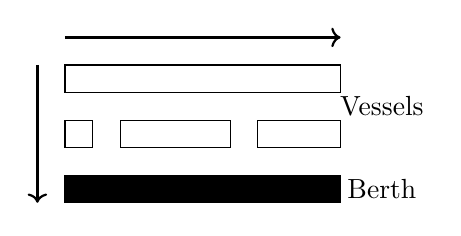
\begin{tikzpicture}[scale=0.35]
      \draw[rotate=90,fill=black] (0,0) rectangle (1,10);
      \draw[rotate=90](2,0) rectangle (3,3);
      \draw[rotate=90](2,4) rectangle (3,8);
      \draw[rotate=90](2,9) rectangle (3,10);
      \draw[rotate=90](4,0) rectangle (5,10);

      \draw[thick,->] (-11,5)--(-11,0);
      \draw[thick,->] (-10,6)--(0,6);

      \node at (1.5,0.5) {Berth};
      \node at (1.5,3.5) {Vessels};
    \end{tikzpicture}
    \caption{Example of berth allocation. Vessels are docked in berth locations (horizontal) and are queued over time (vertical). The vertical arrow represents the movement direction of queued vessels and the horizontal arrow represents the direction of departure.}
    \label{subfig:bapexample}
  \end{figure}

  \begin{figure}[htpb]
    \centering
    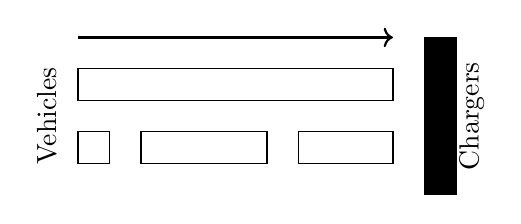
\begin{tikzpicture}[scale=0.4]
      \draw[fill=black] (0,0) rectangle (1,5);

      \draw[rotate=90](1,1) rectangle (2,4);
      \draw[rotate=90](1,5) rectangle (2,9);
      \draw[rotate=90](1,10) rectangle (2,11);
      \draw[rotate=90](3,1) rectangle (4,11);

      \draw[thick,->] (-11,5)--(-1,5);

      \node[rotate=90] at (-12,2.5) {Vehicles};
      \node[rotate=90] at (1.5,2.5) {Chargers};
    \end{tikzpicture}
    \caption{Example of position allocation. Vehicles are placed in queues to be charged and move in the direction indicated by the arrow.}
    \label{subfig:papexample}
  \end{figure}


%%--------------------------------------------------------------------------------
% Variable table
\begin{table}[!htpb]
  \caption{Notation used throughout the paper}
  \label{tab:variables}
  \centering
  \begin{tabularx}{\textwidth}{l l}
    \toprule
    \textbf{Variable} & \textbf{Description}                                                                               \\
    \toprule
    \multicolumn{2}{l}{Input values}                                                                                       \\
    $n_B$        & Number of buses                                                                                         \\
    $M$          & An arbitrary very large upper bound value                                                               \\
    $n_V$        & Number of total visits                                                                                  \\
    $n_Q$        & Number of queues                                                                                        \\
    $n_C$ 	 & Number of chargers                                                                                      \\
    $\mathbb{V}$ & Set of visit indices, $\mathbb{V} = \{1, ..., n_V\}$                                                    \\
    $\mathbb{B}$ & Set of bus indices, $\mathbb{B} = \{1, ..., n_B\}$                                                      \\
    $\mathbb{Q}$          & Set of queue indices, $\mathbb{Q} = \{1, ..., n_Q\}$                                                             \\
    $i,j$        & Indices used to refer to visits                                                                         \\
    $b$ 	 & Index used to refer to a bus                                                                            \\
    $q$ 	 & Index used to refer to a queue                                                                          \\
    \hline
    \multicolumn{2}{l}{Problem definition parameters}                                                                      \\
    $\Gamma$   & $\Gamma: \mathbb{V} \rightarrow \mathbb{B}$ with $\Gamma_i$ used to denote the bus for visit $i$                                   \\
    $\alpha_i$ & Initial charge percentage time for visit $i$                                                                   \\
    $\beta_i$ & Final charge percentage for bus $i$ at the end of the time horizon                                             \\
    $\epsilon_q$ & Cost of using charger $q$ per unit time                                                                        \\
    $\Upsilon$   & $\Upsilon: \mathbb{V} \rightarrow \mathbb{V}$ mapping a visit to the next visit by the same bus with $\Upsilon_i$ being the shorthand. \\
    $\kappa_b$ & Battery capacity for bus $b$                                                                                   \\
    $\lambda_i$ & Discharge of visit over route $i$                                                                              \\
    $\nu_b$ & Minimum charge allowed for bus $b$                                                                             \\
    $\tau_i$ & Time visit $i$ must depart the station                                                                         \\
    $\zeta_b$ & Discharge rate for bus $b$                                                                                     \\
    $a_i$ & Arrival time of visit  $i$                                                                                     \\
    $i_0$ & Indices associated with the initial arrival for every bus in $A$                                               \\
    $i_f$ & Indices associated with the final arrival for every bus in $A$                                                 \\
    $m_q$ & Cost of a visit being assigned to charger $q$                                                                  \\
    $r_q$ & Charge rate of charger $q$ per unit time                                                                       \\
    \hline
    \multicolumn{2}{l}{Decision Variables}                                                                                 \\
    $\delta_{ij}$ & Binary variable determining temporal ordering of vehicles $i$ and $j$                                       \\
    $\eta_i$    & Initial charge for visit $i$                                                                                \\
    $\sigma_{ij}$ & Binary variable determining the queue ordering between vehicles $i$ and $j$                                 \\
    $c_i$    & Ending charge time for visit $i$                                                                            \\
    $g_{iq}$ & The charge gain for visit $i$ from charger $q$                                                              \\
    $p_i$    & Amount of time spent on charger for visit $i$                                                               \\
    $u_i$    & Starting charge time of visit $i$                                                                           \\
    $v_i$    & Assigned queue for visit $i$                                                                                \\
    $w_{iq}$ & Binary assignment variable for visit $i$ to queue $q$                                                       \\
    \bottomrule
  \end{tabularx}
\end{table}


%%--------------------------------------------------------------------------------
% Berth spatio-temporal graph
\begin{figure}[htbp]
	\centerline{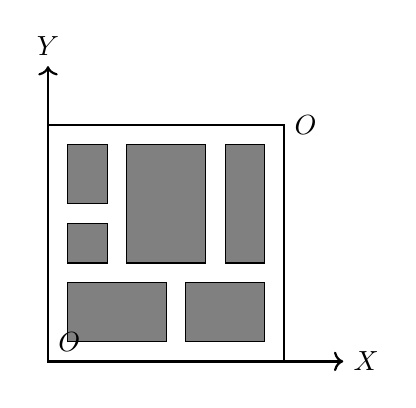
\begin{tikzpicture}[scale=0.25]
	    \draw [thick, -] (0,0) rectangle (12,12) node[right]{$O$};
	    \draw[fill=gray] (1,1) rectangle (6,4);
	    \draw[fill=gray] (11,11) rectangle (9,5);
	    \draw[fill=gray] (8,11) rectangle (4,5);
	    \draw[fill=gray] (1,11) rectangle (3,8);
	    \draw[fill=gray] (1,7) rectangle (3,5);
	    \draw[fill=gray] (11,1) rectangle (7,4);
        \draw [thick,<->] (0,15) node[above]{$Y$}                      --
                                 (0,0)node[above right]{$\mathbb{O}$} --
                                 (15,0) node[right]{$X$};
	\end{tikzpicture}}
	\caption{Example of rectangle packing problem}
	\label{fig:packexample}
\end{figure}

%%--------------------------------------------------------------------------------
% Spatial temporal graph representation
\begin{figure}[ht]
	\centerline{
	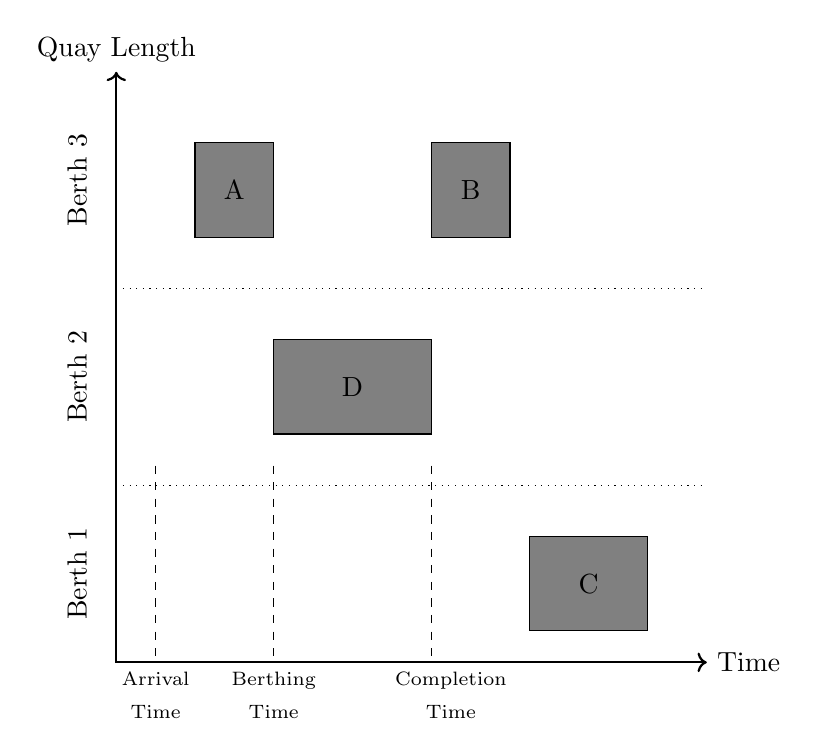
\begin{tikzpicture}[scale=0.5]
        \draw [thick,<->] (0,15) node[above]{Quay Length} --
                                 (0,0)                    --
                                 (15,0) node[right]{Time};
        \node[rectangle, draw, fill=gray, minimum width=1cm, minimum height = 1.2cm] at (3,12) {A};
        \node[rectangle, draw, fill=gray, minimum width=1cm, minimum height = 1.2cm] at (9,12) {B};
        \node[rectangle, draw, fill=gray, minimum width=2cm, minimum height = 1.2cm] at (6,7) {D};
        \node[rectangle, draw, fill=gray, minimum width=1.5cm, minimum height = 1.2cm] at (12,2) {C};

	\node [below,align=center] at (1.0,0) {\scriptsize Arrival\\ \scriptsize Time};
	\draw[dashed] (1.0,5)--(1.0,0);

	\node [below, align=center] at (4,0) {\scriptsize Berthing\\ \scriptsize Time};
	\draw[dashed] (4,5)--(4,0);

	\node [below, align=center] at (8.5,0) {\scriptsize Completion\\ \scriptsize Time};
	\draw[dashed] (8,5)--(8,0);

        \draw[dotted] (0, 4.5) -- (15, 4.5);
        \draw[dotted] (0, 9.5) -- (15, 9.5);

	\node[rotate=90] at (-1, 2.25) {Berth 1};
	\node[rotate=90] at (-1, 7.25) {Berth 2};
	\node[rotate=90] at (-1, 12.25) {Berth 3};

	\end{tikzpicture}
    }
	\caption{The representation of the berth-time space}
	\label{fig:bap}
\end{figure}

%%--------------------------------------------------------------------------------
%
\begin{figure}[htbp]
	\centerline{
	\begin{tikzpicture}[scale=0.35]
		\draw [thick,<->] (0,15) node[above]{Quay Length} --
					 (0,0)                                   --
					 (15,0) node[right]{Time};

		\node[rectangle, draw, minimum width=1.5cm, minimum height = 2cm] at (5,8) {$i$};
		\node[rectangle, draw, minimum width=1cm, minimum height = 1cm] at (2,2) {$j$};
		\node[rectangle, draw, dashed, minimum width=1cm, minimum height = 1.2cm] at (5,12) {$k_1$};
		\node[rectangle, draw, dashed, minimum width=1cm, minimum height = 1.2cm] at (7,6) {$k_3$};
		\node[rectangle, draw, dashed, minimum width=1cm, minimum height = 1.2cm] at (4,2) {$k_2$};
	\end{tikzpicture}
	}
	\caption{Examples of different methods of overlapping. Space overlap: $v_{k_1} < v_{i} + s_i \therefore \delta_{k_{1}i} = 0$.
          Time overlap $u_{k_1} < u_{j} + p_j \therefore \sigma_{k_{2}j} = 0$. Both space and time overlap $\sigma_{k_{3}i} = 0$ and
          $\delta_{k_{3}j} = 0$.}
	\label{fig:multipleassign}
\end{figure}

%%--------------------------------------------------------------------------------
% Charge Schedule
\pgfplotstableread[col sep = comma]{fig/data/qm-schedule.csv}\scheduledataquin
\pgfplotstableread[col sep = comma]{fig/data/milp-schedule.csv}\scheduledatamilp

\begin{subfigures}
    % Quin ----------
    \begin{figure}[htpb]
        \centering
        \begin{tikzpicture}[scale=0.65]
        \pgfplotstablegetcolsof{\scheduledataquin}
        \pgfmathtruncatemacro\NumCols{\pgfplotsretval/3 - 1}
        \begin{axis}[title={Quin Schedule},
                     xlabel={Time [hr]}, ylabel={Active charge times},
                     xmin=0, xmax=24]
            \foreach \i in {0, ..., \NumCols}
            {
                \pgfmathsetmacro{\v}{\fpeval{3*\i} + 0}
                \pgfmathsetmacro{\u}{\fpeval{3*\i} + 1}
                \pgfmathsetmacro{\p}{\fpeval{3*\i} + 2}
                \addplot +[only marks, error bars/.cd, x dir=plus, x explicit] table[x index=\u, x error index=\p, y index =\v]{\scheduledataquin};
            }
        \end{axis}
        \end{tikzpicture}
        \caption{Charging schedule generated by Quin Modified algorithm.}
        \label{subfig:quin-schedule}
    \end{figure}
    \hfill
    % MILP ----------
    \begin{figure}[htpb]
        \centering
        \begin{tikzpicture}[scale=0.65]
        \pgfplotstablegetcolsof{\scheduledatamilp}
        \pgfmathtruncatemacro\NumCols{\pgfplotsretval/3 - 1}
        \begin{axis}[title={MILP Schedule},
                     xlabel={Time [hr]}, ylabel={Active charge times},
                     xmin=0, xmax=24]
            \foreach \i in {0, ..., \NumCols}
            {
                \pgfmathsetmacro{\v}{\fpeval{3*\i} + 0}
                \pgfmathsetmacro{\u}{\fpeval{3*\i} + 1}
                \pgfmathsetmacro{\p}{\fpeval{3*\i} + 2}
                \addplot +[only marks, error bars/.cd, x dir=plus, x explicit] table[x index=\u, x error index=\p, y index =\v]{\scheduledatamilp};
            }
        \end{axis}
        \end{tikzpicture}
    \caption{Charging schedule generated by MILP PAP algorithm.}
    \label{subfig:milp-schedule}
    \end{figure}
\end{subfigures}


%%--------------------------------------------------------------------------------
% Bus charges
\pgfplotstableread[col sep = comma]{fig/data/qm-charge.csv}\chargedataquin
\pgfplotstableread[col sep = comma]{fig/data/milp-charge.csv}\chargedatamilp

\begin{subfigures}
    % Quinn ----------
    \begin{figure}[htpb]
        \centering
        \begin{tikzpicture}[scale=0.65]
        \pgfplotstablegetcolsof{\chargedataquin}
        \pgfmathtruncatemacro\NumCols{\pgfplotsretval/2-1} 
        \begin{axis}[title={Quin Charges},
                     xlabel={Time [hr]},
                     xmin=0, xmax=24,
                     ylabel={Charge [kwh]}]
            \foreach \i in {0, ..., \NumCols}
            {
                \pgfmathsetmacro{\u}{\fpeval{2*\i} + 0}
                \pgfmathsetmacro{\etas}{\fpeval{2*\i} + 1}
                \addplot +[mark=none] table[x index=\u, y index =\etas]{\chargedataquin};
            }
        \end{axis}
        \end{tikzpicture}
    \caption{Bus charges for the Quin Modified charging schedule. The charging scheme of the Quin charger is more predictable during the working day.}
    \label{subfig:quin-charge}
    \end{figure}
    \hfill
    % MILP ----------
    \begin{figure}[htpb]
        \centering
        \begin{tikzpicture}[scale=0.65]
        \pgfplotstablegetcolsof{\chargedataquin}
        \pgfmathtruncatemacro\NumCols{\pgfplotsretval/2-1} 
        \begin{axis}[title={MILP Charges},
                     xlabel={Time [hr]},
                     xmin=0, xmax=24,
                     ylabel={Charge [kwh]}]
            \foreach \i in {0, ..., \NumCols}
            {
                \pgfmathsetmacro{\u}{\fpeval{2*\i} + 0}
                \pgfmathsetmacro{\etas}{\fpeval{2*\i} + 1}
                \addplot +[mark=none] table[x index=\u, y index =\etas]{\chargedatamilp};
            }
        \end{axis}
        \end{tikzpicture}
    \label{subfig:milp-charge}
    \caption{The bus charges for the MILP PAP charging schedule. The MILP model allows for guarantees of minimum/maximum changes during the working day as well as charges at the end of the day.}
    \label{subfig:milp-charge}
    \end{figure}
\end{subfigures}

%%--------------------------------------------------------------------------------
% Power consumption
\pgfplotstableread[col sep = comma]{fig/data/qm-power-usage.csv}\powerdataquin
\pgfplotstableread[col sep = comma]{fig/data/milp-power-usage.csv}\powerdatamilp

\begin{figure}
    \centering
    \begin{tikzpicture}[scale=0.65]
    \begin{axis}[title={Power Usage},
                 xlabel={Time [hr]}, ylabel={Power Usage [kw]},
                 xmin=4, xmax=24, ymin=0]
        % Quin ----------
        \addplot[blue!80!black, fill=blue, fill opacity=0.25, no markers]
                     table[x=time, y=power] {\powerdataquin};
        \addlegendentry{Quin}

        % MILP ----------
        \addplot[red!80!black, fill=red, fill opacity=0.25, no markers]
                    table[x=time, y=power] {\powerdatamilp};
        \addlegendentry{MILP}
    \end{axis}
    \end{tikzpicture}
\caption{Total accumulated energy consumed by the Quin-Modified and MILP schedule throughout the time horizon.}
\label{fig:power-usage}
\end{figure}


%%--------------------------------------------------------------------------------
% Power consumption
\pgfplotstableread[col sep = comma]{fig/data/qm-acc-energy-usage.csv}\accenergydataquin
\pgfplotstableread[col sep = comma]{fig/data/milp-acc-energy-usage.csv}\accenergydatamilp

\begin{figure}
    \centering
    \begin{tikzpicture}[scale=0.65]
    \begin{axis}[title={Accumulated Energy Usage},
                 xlabel={Time [hr]}, ylabel={Energy Usage [Kwh]},
                 xmin=4, xmax=24, ymin=0]
        % Quin ----------
        \addplot[blue!80!black, no markers]
                     table[x=time, y=power] {\accenergydataquin};
        \addlegendentry{Quin}

        % MILP ----------
        \addplot[red!80!black, no markers]
                    table[x=time, y=power] {\accenergydatamilp};
        \addlegendentry{MILP}
    \end{axis}
    \end{tikzpicture}
\caption{Amount of power consumed by Quin-Modified and MILP schedule over the time horizon.}
\label{fig:energy-usage}
\end{figure}


%%--------------------------------------------------------------------------------
% Charger usage count
\pgfplotstableread[col sep = comma]{fig/data/qm-charge-cnt.csv}\usagedataquin
\pgfplotstableread[col sep = comma]{fig/data/milp-charge-cnt.csv}\usagedatamilp

\begin{subfigures}
    % Fast ----------
    \begin{figure}[htpb]
        \centering
        \begin{tikzpicture}[scale=0.65]
        \begin{axis}[title={Fast Charger Usage},
                     xlabel={Time [hr]},ylabel={Count},
                     xmin=0, xmax=24,
                     ytick distance=1]
            \addplot[blue!80!black, fill=blue, fill opacity=0.25, no markers] table[x=visit, y=fast] {\usagedataquin};
            \addlegendentry{Quin}
            \addplot[red!80!black, fill=red, fill opacity=0.5, no markers] table[x=visit, y=fast] {\usagedatamilp};
            \addlegendentry{MILP}
        \end{axis}
        \end{tikzpicture}
    \caption{Number of fast chargers for Quin and MILP PAP.}
    \label{fig:fast-charger-usage}
    \end{figure}
    \hfill
    % Slow ----------
    \begin{figure}[htpb]
        \centering
        \begin{tikzpicture}[scale=0.65]
        \begin{axis}[title={Slow Charge Usage},
                     xlabel={Time [hr]},ylabel={Count},
                     xmin=0, xmax=24,
                     ytick distance=1]
            \addplot[blue!80!black, fill=blue, fill opacity=0.25, no markers] table[x=visit, y=slow] {\usagedataquin};
            \addlegendentry{Quin}
            \addplot[red!80!black, fill=red, fill opacity=0.15, no markers] table[x=visit, y=slow] {\usagedatamilp};
            \addlegendentry{MILP}
        \end{axis}
        \end{tikzpicture}
    \caption{Number of slow chargers for Quin and MILP PAP.}
    \label{fig:slow-charger-usage}
    \end{figure}%
\end{subfigures}


%%%%%%%%%%%%%%%%%%%%%%%%%%%%%%%%%%%%%%%%%%%%%%%%%%%%%%%%%%%%%%%%%%%%%%%%%%%%%%%%%
\end{document}